\documentclass[12pt,letterpaper]{article}
\usepackage[left=1in,right=1in,top=1in,bottom=1in]{geometry}
\usepackage[utf8]{inputenc}
\usepackage{afterpage}
\usepackage{xcolor}
\setlength{\emergencystretch}{3em} % prevent overfull lines
\providecommand{\tightlist}{%
\setlength{\itemsep}{0pt}\setlength{\parskip}{0pt}}

\usepackage[hidelinks,bookmarks]{hyperref}
\usepackage{bookmark}
\usepackage[compact]{titlesec}
\usepackage[title]{appendix}
\usepackage{graphicx}
\usepackage{enumitem}
\usepackage{dirtytalk}
\usepackage[
	backend=bibtex,
	sorting=none,
]{biblatex}
\addbibresource{biblio.bib}

\setlength{\parindent}{0em}
\setlength{\parskip}{1em}
\setlength{\footnotesep}{1em}

\urlstyle{same}

\title{Decentralized Social Networking Protocol (DSNP)}
\author{
	Project Liberty\\
	\href{mailto:hello@dsnp.org}{hello@dsnp.org}\\
	\url{projectliberty.io} \url{dsnp.org}
}
\date{\textit{Originally Released}\\
October 2020\\
\textit{Revised Edition}\\
March 2024}

\begin{document}

\maketitle

\begin{abstract}
	The decentralized social networking protocol (DSNP) allows users to interact via a global,
	open, decentralized social graph, giving them control of their identities and personal data
	while avoiding the balkanization of the current social network
	platforms and creating an open ecosystem of network participants. We propose a protocol
	for writing and reading social network data on public consensus systems.
	This protocol defines how identity, social graph, and messaging elements are represented
	to create a decentralized social network. Applicable aspects of control, privacy,
	authenticity, portability, usability, and extensibility are addressed for each element.
	This paper is accompanied by a protocol specification document.\footnote{https://spec.dsnp.org}
\end{abstract}

\vfill
\copyright\, 2020-2024 Project Liberty\\
Published under a Creative Commons Attribution-ShareAlike 4.0 License.\\
See \textit{https://creativecommons.org/licenses/by-sa/4.0/} for details.

% Remove the page number from the title page and start numbering at 1 on the second page
\thispagestyle{empty}
\clearpage

\raggedright

\section*{Preface to the Revised Edition}

In the several years since this white paper was first published, consensus systems---as
represented by blockchains, distributed ledger systems, and other technologies---have
continued to evolve rapidly, benefiting from both an increase in public interest and renewed
enthusiasm from the worldwide academic and development communities. There has been a
corresponding, and welcome, shift away from a seemingly single-minded focus on
cryptocurrency and financialization toward a more nuanced idea of a world of decentralized
identity and decentralized applications (dApps). While some discussion of economic
incentives is unavoidable, and indeed important, for consensus systems to endure and thrive,
this shift has helped to create a technological environment where the benefits of
decentralization and consensus-based state management have been recognized as extending far
beyond purely financial applications. This in turn has helped to usher in new language that
allows us to speak about such systems in more inclusive terms: whereas the first edition of
this paper referenced the well known blockchain smart contract paradigm specifically, we
can, with the benefit of time and hindsight, address the protocol more generally in terms of
consensus systems, shared state, and the invocation of operations and resulting state change
records on these systems.

In preparing this revised edition, we have tried to avoid radical alterations to the original
text; as such, this work can be viewed as both a historical document of the thought
processes and design decisions that shaped the protocol initially, and as a statement of the
objectives and design principles that should continue to be applied to the protocol's future
evolution. With that in mind, it is worth pointing out that some specific terminology or
implementation strategies may now be different in the official DSNP specification (which did
not exist when this white paper was first published). Where explanation is needed, we have
provided footnotes to address the current state of protocol evolution and divergence from
the initial proposal (such as the change from incremental Graph Change Events to bulk
changes via a User Data management paradigm) but have kept the historical text as intact as
possible, as in almost all cases the same concepts still apply, even if implementation
strategies have changed. Finally, we have moved the section on Batch Announcements from the
appendix to be its own core section. This reflects its importance for implementing DSNP
systems that are economically viable and highly scalable.

\clearpage
\section{Introduction}\label{sec:introduction}

Most people have come to rely predominantly on private platforms serving as trusted third
parties to manage and facilitate communication with their broadest network of
relationships. This network is commonly known as a \say{social graph,} and presently most
social graphs are privately owned and controlled by a small number of large technology
companies. While the current ecosystem of social graphs has pioneered a new way for people
to interact with their personal network and public figures on an unprecedented scale, it
suffers from inherent weaknesses related to trust, incentive models, and equitable
participation in the attention economy.

These large, corporate-owned social graphs have made it possible for people to expand
their network of relationships to an extremely large scale. However, each social graph is
isolated, locking in users as a result of the high cost of re-creating a social graph in
another provider's \say{walled garden.} This balkanized environment also prevents the
broader developer community from helping to address challenging problems or contributing
new innovations to improve this pervasive technology.

All major social networks employ personalization algorithms to determine what content is
presented to users. These are centralized, usually closed algorithms that are opaque and
proprietary, and they offer the user limited input or insight into how they operate.
Through passive data collection, these algorithms often trigger users' negative,
fight-or-flight reactions to increase engagement.\cite{psychology_today_2017}

This approach, in turn, creates more advertising opportunities and drives more revenue to
the large companies that control the largest social graphs. Malicious actors exploit these
algorithms by deploying bots, artificial profiles, and divisive content to manipulate users
at scale.

What is needed is a universally accessible, unified, and decentralized social graph that
allows developers to build an ecosystem with a variety of applications. By decoupling
applications and data, this ecosystem will allow for a wide range of personalization
algorithms to be developed and employed by different applications, and even applied to
specific communities and topics.

This new approach will enable users to move seamlessly between applications without
rebuilding their network of friends and public figures at each destination. Further, users
will be able to choose from a diverse set of recommendation and moderation systems.
Unbundling the social graph will lower switching costs and allow for a marketplace where
developers compete on a level playing field, with diverse winners based on user needs and
preferences.


In this paper, we propose a solution to the balkanization of social graphs by employing a
public protocol for writing and reading social graph data on public consensus systems using
data transactions. We include both a structure for the graph as well as the mechanism for
creating authentic claims from and about the user. Further, we outline an approach to
sharing content over such a social graph, and ways in which new services can be built to
efficiently aggregate and disseminate such information on public consensus systems at the
scale required for a universal decentralized graph to be adopted by the majority of the
population.

\section{Solution Overview}\label{sec:solution_overview}

The decentralized social networking protocol (DSNP) is composed of three major elements.
The first is identity, which creates a representation of users. The second is a social
graph, which models relationships between user identities. The final element is messaging,
which facilitates communication between the users based on their social graph connections.

\begin{samepage}
	We considered many different design aspects when creating the elements of
	this protocol. Six core aspects we address are:

	\begin{description}
		\tightlist
		\item[Agency:]
		      Who owns and controls the data?
		\item[Privacy:]
		      How and when is data private, and how is that privacy managed?
		\item[Authenticity:]
		      How can protocol actions be verified and attributed?
		\item[Portability:]
		      How can users make use of their personal data in different contexts?
		      What data is available to third parties and how is it obtained?
		\item[Usability:]
		      What options exist for user interaction?
		\item[Extensibility:]
		      How is functionality changed or upgraded over time?
	\end{description}
\end{samepage}

Most social networking products solve only some of these aspects, whether through technical
limitations or explicit choices. Vertically integrated products inherently struggle with
portability, and many choose not to enforce privacy or ownership standards. Federated
protocols, with their dependence on shared servers, generally can't provide strong user data
ownership guarantees. Existing decentralized networks have limited privacy and private
communication capabilities and struggle with usability, often coupling the ability to exercise
core social functionality with transaction fees denominated in a specific cryptocurrency token.
We believe the optimal approach to
address these six core aspects is a protocol that leverages an existing public consensus
system as a neutral, decentralized platform for data and communications, while defining a
standard format for data interaction and employing strong encryption for privacy, allowing
any number of different user experiences to be created.

DSNP models the identity of a user as individually owned shared state on a public consensus
system. Protocol operations allow the user to maintain complete control of their data, and
ensure that no third party can revoke their access. These data transactions also act as the
root for other protocol actions, allowing user relationships, messages, and content to have
a common attribution. The operations enable users to delegate permissions for certain
actions in the protocol to third parties, such as user agents or applications, without
sacrificing ownership and control. Delegation allows for cost shifting, so authorized
delegates can pay for the calls they invoke on the user's behalf.  A \say{design by
  contract} approach allows for functional upgrades and multiple different implementations,
while preserving user discretion on when or if to make changes.

The social graph is composed of events emitted on a consensus system, modeling a directed
graph of \say{follow} relationships. Users have direct control to make changes on the graph
independent of the provider they are using. Relationships can be public or private,
including the indication of whether the event is starting or ending a relationship. By using
a common data format on a consensus system, the data has inherent portability. Users decide
whom they share their data with, instead of being locked in to a third-party system. As with
identity, users can delegate permissions to a user agent or third party, allowing them to
emit relationship events on their behalf. In addition, users can share encryption keys to
give third parties the ability to read private graph data. The protocol also supports
extending relationship types to support other use cases, such as friends, fans, or group
membership.

Messaging is modeled as broadcast event announcements on a consensus system that link to
content stored on a public file server. The solution supports options for both message and
recipient privacy. All message data, whether stored on or off the chain, has a cryptographic
chain of trust back to the originating identity. Since all messages are announced on chain,
the common data format allows messages to be retrieved by any conforming client or third
party, although private messages require the appropriate keys to decrypt them. Users can
also delegate permissions to send messages on their behalf, whether for usability or
cost-shifting reasons. Finally, the types and formats of messages and message announcements
can be expanded over time to support additional use cases, such as reactions, spam scoring,
curated topics, or tag-based discovery.

Combined, these elements represent an unbundling of social networks as they currently
exist, and create a unified, universally accessible, and decentralized ecosystem for
social activity at global scale.

\section{Identity}\label{sec:identity}

In any social network, users must be consistently identified to engage in most use cases.
The protocol defines a concept of identity to represent users in social graph relationships
called a Social Identity. Social Identities are pseudonymous,\cite{anon_terminology} user
owned, and default private. These properties are essential to the user's overall control of
their identity. Protocol operations define the interface for interaction with the user's
data, standardizing both how users can share their data with others and how they can
delegate certain rights to others to act on their behalf.

\subsection{Pseudonymity}\label{sec:pseudonymity}

DSNP requires Social Identities to be pseudonymous. These identities provide a consistent
record of an online actor not directly tied to an offline identity. To implement
pseudonymity, the data that represents a Social Identity is owned by an anonymous control
key, which allows a user to provide cryptographic proof of ownership. A person may share one
Social Identity across multiple contexts, such as family, business, and gaming, or create
multiple identities to keep different facets of life separate. Each Social Identity is tied
to a separate uncorrelated control key and stored in a user's digital wallet.

\begin{figure}
	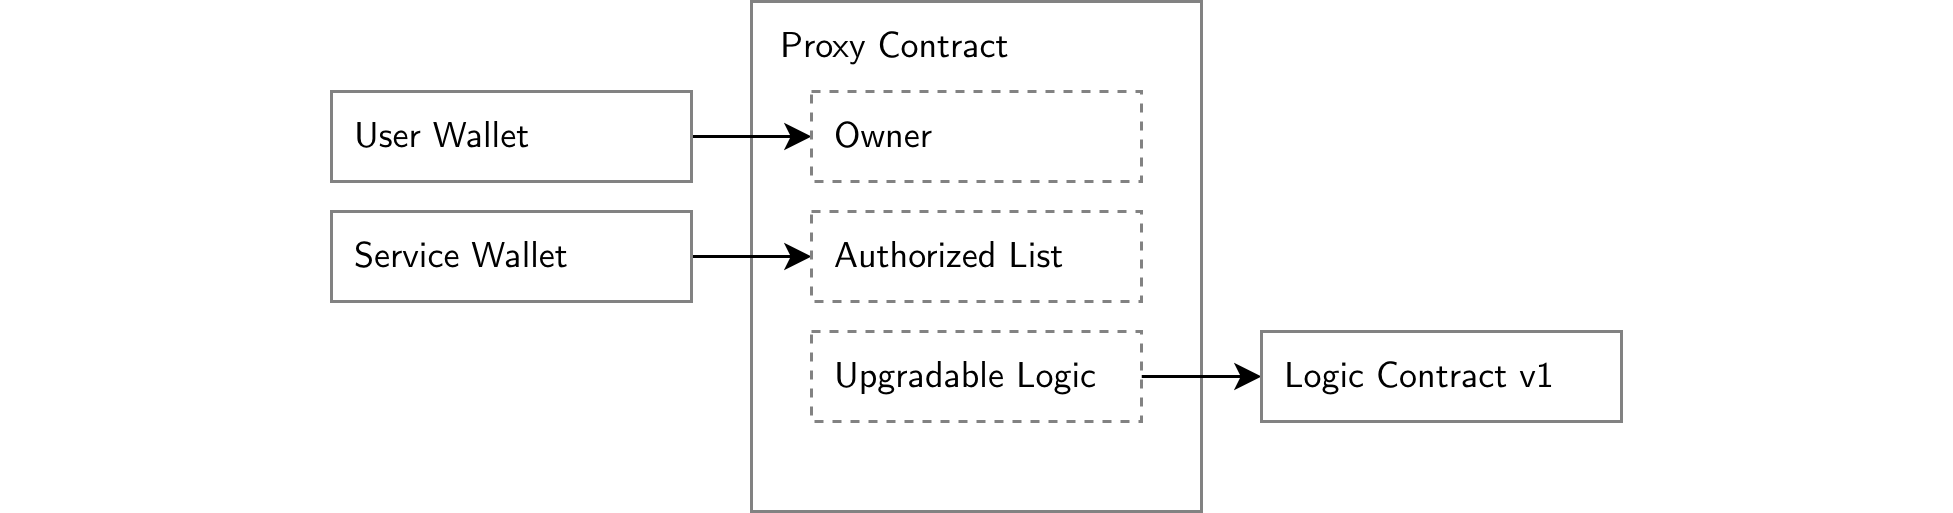
\includegraphics[width=\linewidth]{figures/Social Identity Ownership Structure.png}
	\caption{Social Identity Ownership Structure}
	\label{fig:1}
\end{figure}

\subsection{User Agency and Delegation}\label{sec:user_ownership and_delegation}

With most existing social networks, a user's access to their account can be suspended or
revoked unilaterally by the site owner, based on any number of actual or perceived
behaviors, resulting in the user's loss of access to their personal data and social graph.
Even though the user populated their account with data and social connections, the site
usually owns the account that the user created. A key goal of the protocol is for users to
control and have agency over their data. Three techniques are used to ensure that people control
their Social Identity: direct data control, rights delegation, and identity verification.

\subsubsection{Direct Data Control}

Many blockchain-based projects that employ smart contracts use a single contract instance to
store multiple user's rights. While this approach works for simple use cases, such
as nonupgradable smart contracts associating ERC-20\cite{erc20} token values with unique
addresses, storing multiple users' data in a single smart contract means someone other than
each user has the right to upgrade the common contract. Whoever has upgrade rights
ultimately controls the contract, and therefore the functionality of the contract and the
data it stores.\footnote{The first edition of this paper argued for giving users choice in
  how and when to upgrade their Social Identity as represented specifically by a blockchain
  smart contract. Further research and development led to the conclusion that creating a
  coherent public space would only be possible if the participants agreed to follow the same
  version (with allowances for forward and backward compatibility) of the protocol. The text
  has been updated to reinforce the important role that user opt-in still plays, but that it
  may be implemented using a variety of approaches.} Instead, the protocol guarantees that
each user's control key retains sole control of their personal data and social graph.

One major ramification of direct control is that the user should always have agency in the
adoption of new system logic (for example, smart contract upgrades or blockchain core logic
upgrades). At minimum, users require the ability to opt out of their association with a
given consensus system. Ideally, consensus systems will enable democratic participation in
the governance and adoption of logic related to this protocol; the precise mechanisms that
help achieve this (DAOs, co-ops, etc.) are an area of active research within the technology
community.  This avoids the case of an outside party having unilateral rights to change the
behavior of the system without the user's consent. An outside party in possession of
unilateral access rights would be equivalent to the status quo, meaning that existing social
network providers have the power to revoke user account access. For a Social Identity, no
third party has this capability, within the constraints of the consensus system it is built on.

The \say{design by contract} approach provides another extension to control: complete
implementation change. Although we expect most users to use the same implementation, other
implementations may arise to cover unique use cases since the protocol is designed to be
interface first.

\subsubsection{Rights Delegation}

A Social Identity allows users to delegate certain rights to third parties to act on their
behalf. This ability is accomplished by creating a system to delegate trust using the user's
control key as owner and sole authority to grant new permissions. All granted permissions
can be revoked in the same fashion. Both actions are simply protocol operations.

The delegation of rights never removes the user's agency over their Social Identity. When
delegating rights, it is also possible to limit third-party access to specific actions.
Though third-party \say{bad actors} who receive rights may be able to take actions on the
user's behalf until access is revoked, they cannot escalate their actions to ownership
rights.

Rights delegation also allows for cost shifting. Most blockchains, for example, have
transaction processing costs associated with smart contract invocations. By allowing a third
party to invoke actions on behalf of a user, the user---without sacrificing ownership---can
benefit from the third party's payment of the transaction fee associated with the
invocation. A simple example would be an ad-supported social networking client that pays the
transaction fee for a user when posting a new image or video.

This concept can also be extended to Social Identity creation by having the user sign a
request with the private key from their digital wallet, authorizing a Social Identity to be
created on their behalf. This signed request would be passed to a third party, who would
then pay the fee to create a Social Identity, but with the user's control key as the
owner. Such cost shifting is a key element to initial adoption, since it does not require
users to own any cryptocurrency to create or use a Social Identity.

\begin{figure}
	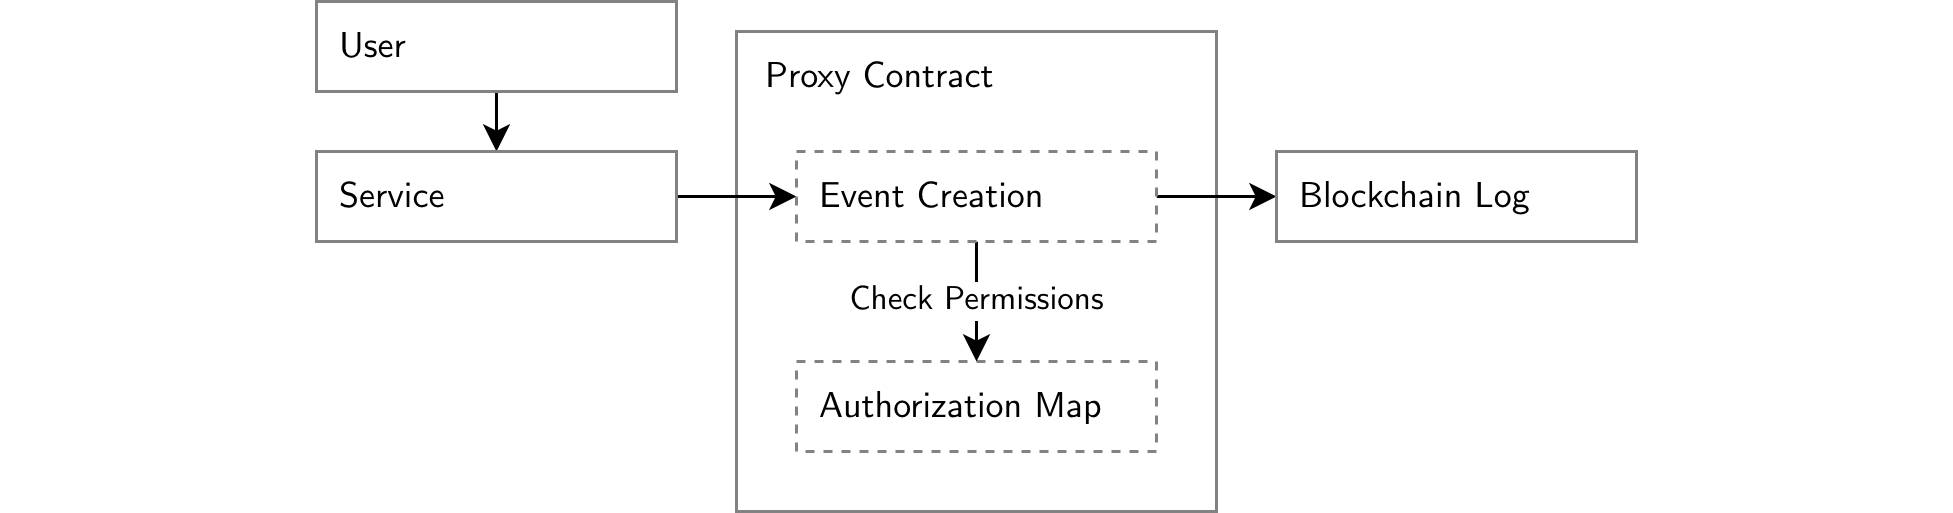
\includegraphics[width=\linewidth]{figures/Cost Shifting.png}
	\caption{Cost Shifting Example}
	\label{fig:2}
\end{figure}

\subsubsection{Identity Verification}

Through rights delegation, some invocations of operations on the user's Social Identity may
be made by third parties. To ensure that only authorized delegates make such calls, all
operations that allow third-party delegate invocations require the third party to be in the
user's authorized list of delegates and to have the sufficient permissions to invoke the
intended action.

Each action on the consensus system taken by an authorized third party can be traced back to
the delegate, verifying the identity of the invoker. Delegates who engage in unauthorized
activity can be identified and their permissions revoked. Actions previously taken by the
abusing party can be refuted by the user.

\subsection{Attributes}\label{sec:attributes}

People using social media often choose to expose parts of their identity, or at least the
identity that they inhabit on social media. Users can attach claims and metadata to their
Social Identity. A set of attributes attached to an identity is often created as a profile:
the most common metadata used on social media are display name and avatar,
but can extend to claims about the user's real-world identity, such as name, age, or
professional certifications. By using this mechanism, services may be created that verify a
user's real identity, similar to Twitter's verified accounts, except open for all to use rather
than only those who Twitter has \say{determined to be an account of public
  interest.}\cite{twitter_verified_accounts}

\subsection{Portability}\label{sec:portability}

When users control their data and it is stored on the consensus system, portability manifests
differently than the traditional export/import paradigm. Data is shared with services
instead of stored in services. People can use more than one service at a time while
continuing to synchronize data between services. While public data is readable by anyone,
private data is controlled through providing a plaintext copy of the data or providing
decryption keys to the service.

As a paradigm for portability, sharing requires the ability of a user to revoke access to a
service that the user no longer desires to use. Two types of data fall outside the
protocol's protections: plaintext copies and public data. When a user shares data with a
service, technical controls in the protocol can no longer protect the user's data.  Instead,
control of that copy of the data is governed by the terms of service and the applicable laws
governing the service. Depending on jurisdiction or other factors, the European Union
General Data Protection Regulation,\cite{gdpr2016} California Consumer Privacy
Act,\cite{ccpa2018} Lei Geral de Proteção de Dados,\cite{lgpd2019} and similar regulations
may provide coverage, but they are outside the scope of the protocol. By definition, public
data is accessible to all and is also governed by local law.

Unlike previously shared data, user control of the creation and sharing of new data is
absolute. The user can stop any undesired plaintext sharing and public data publishing. If
the user has shared a decryption key with a service, the user must change their encryption
key to disable a service's access to new private data.

\section{Social Graph}\label{sec:social_graph}

DSNP provides for the decentralized creation and management of a global mapping of all users
and how they are related. This global mapping is commonly known as a social graph.
Relationships are first-order primitives in the protocol, and they represent connections
between users in a social graph. The two most common relationship types in social networks
are \say{Friend} and \say{Follow.} These relationships represent connections between Social
Identities, and can be public or private. Public relationships can be seen by anyone, while
private relationships allow user control over who can view them.

\subsection{Relationship Types}\label{sec:relationship_types}

Users, represented by Social Identities, are the vertices in the social graph, and
relationships are the edges. These relationships can be directed, such as in a Follow
relationship, or undirected, such as in a Friend relationship. Twitter is an
example of the directed Follow model. A public Follow relationship is created by the
follower, but it does not require the permission of the followed.\footnote{Twitter allows for
  various tweaks to this simplistic model; blocking and privacy options, for example.} The
reciprocal relationship can also exist, but it is not required. The follower controls both
the formation and removal of the relationship. Facebook and LinkedIn are examples of
networks that have an undirected Friend model. This requires the permission of both users to
form the relationship, but either can remove it. DSNP uses Follow-based, directed edges in
its social graph. The undirected Friend relationship, along with other relationship types,
can use this directed approach as a building block for more complex relationship
types. Access to encrypted, private posts requires permission from the user being followed
in order to obtain the appropriate decryption keys, and closely resembles the process of
creating a Friend relationship.

\subsection{Graph Change Events}\label{sec:graph_change_events}

The protocol models the creation or removal of a Follow relationship as a Graph Change
Event.\footnote{Since this paper was originally published, the specification has endorsed
  handling of graph changes by updating shared state in aggregated form via the User Data
  operations. However, from a systems reasoning point of view, viewing changes to the social
  graph as discrete events is still relevant.} The sequence of these events represents the
current state of the social graph rooted at each Social Identity. The event structure allows
some data to be either public or private, even though all events on a public consensus
system are by necessity public. A mechanism is also provided for sharing private event data
with trusted parties.

\subsubsection{Structure}

To create a Follow relationship, the aspiring follower creates a Graph Change Event, with
themselves as the Actor, the Social Identity they want to follow as the Object, and follow
as the Action. The Graph Change Event is then published via a protocol operation on the
user's Social Identity, making it visible on the consensus system.

\begin{samepage}
	Graph Change Events have four major components\footnote{Actor and Object terms are borrowed from the Activity Streams 2.0 Vocabulary\cite{activitypub}}:

	\begin{description}
		\tightlist
		\item[Type:]
		      Whether this is a public or private Graph Change Event.
		\item[Actor:]
		      The Social Identity creating the event. In a public Follow relationship, this would be the follower.
		\item[Object:]
		      The Social Identity that is being linked to the event. In a public Follow relationship, this would be the user being followed or unfollowed.
		\item[Action:]
		      The action being taken. In a public Follow relationship, the options are follow and unfollow.
	\end{description}
\end{samepage}

\begin{figure}
	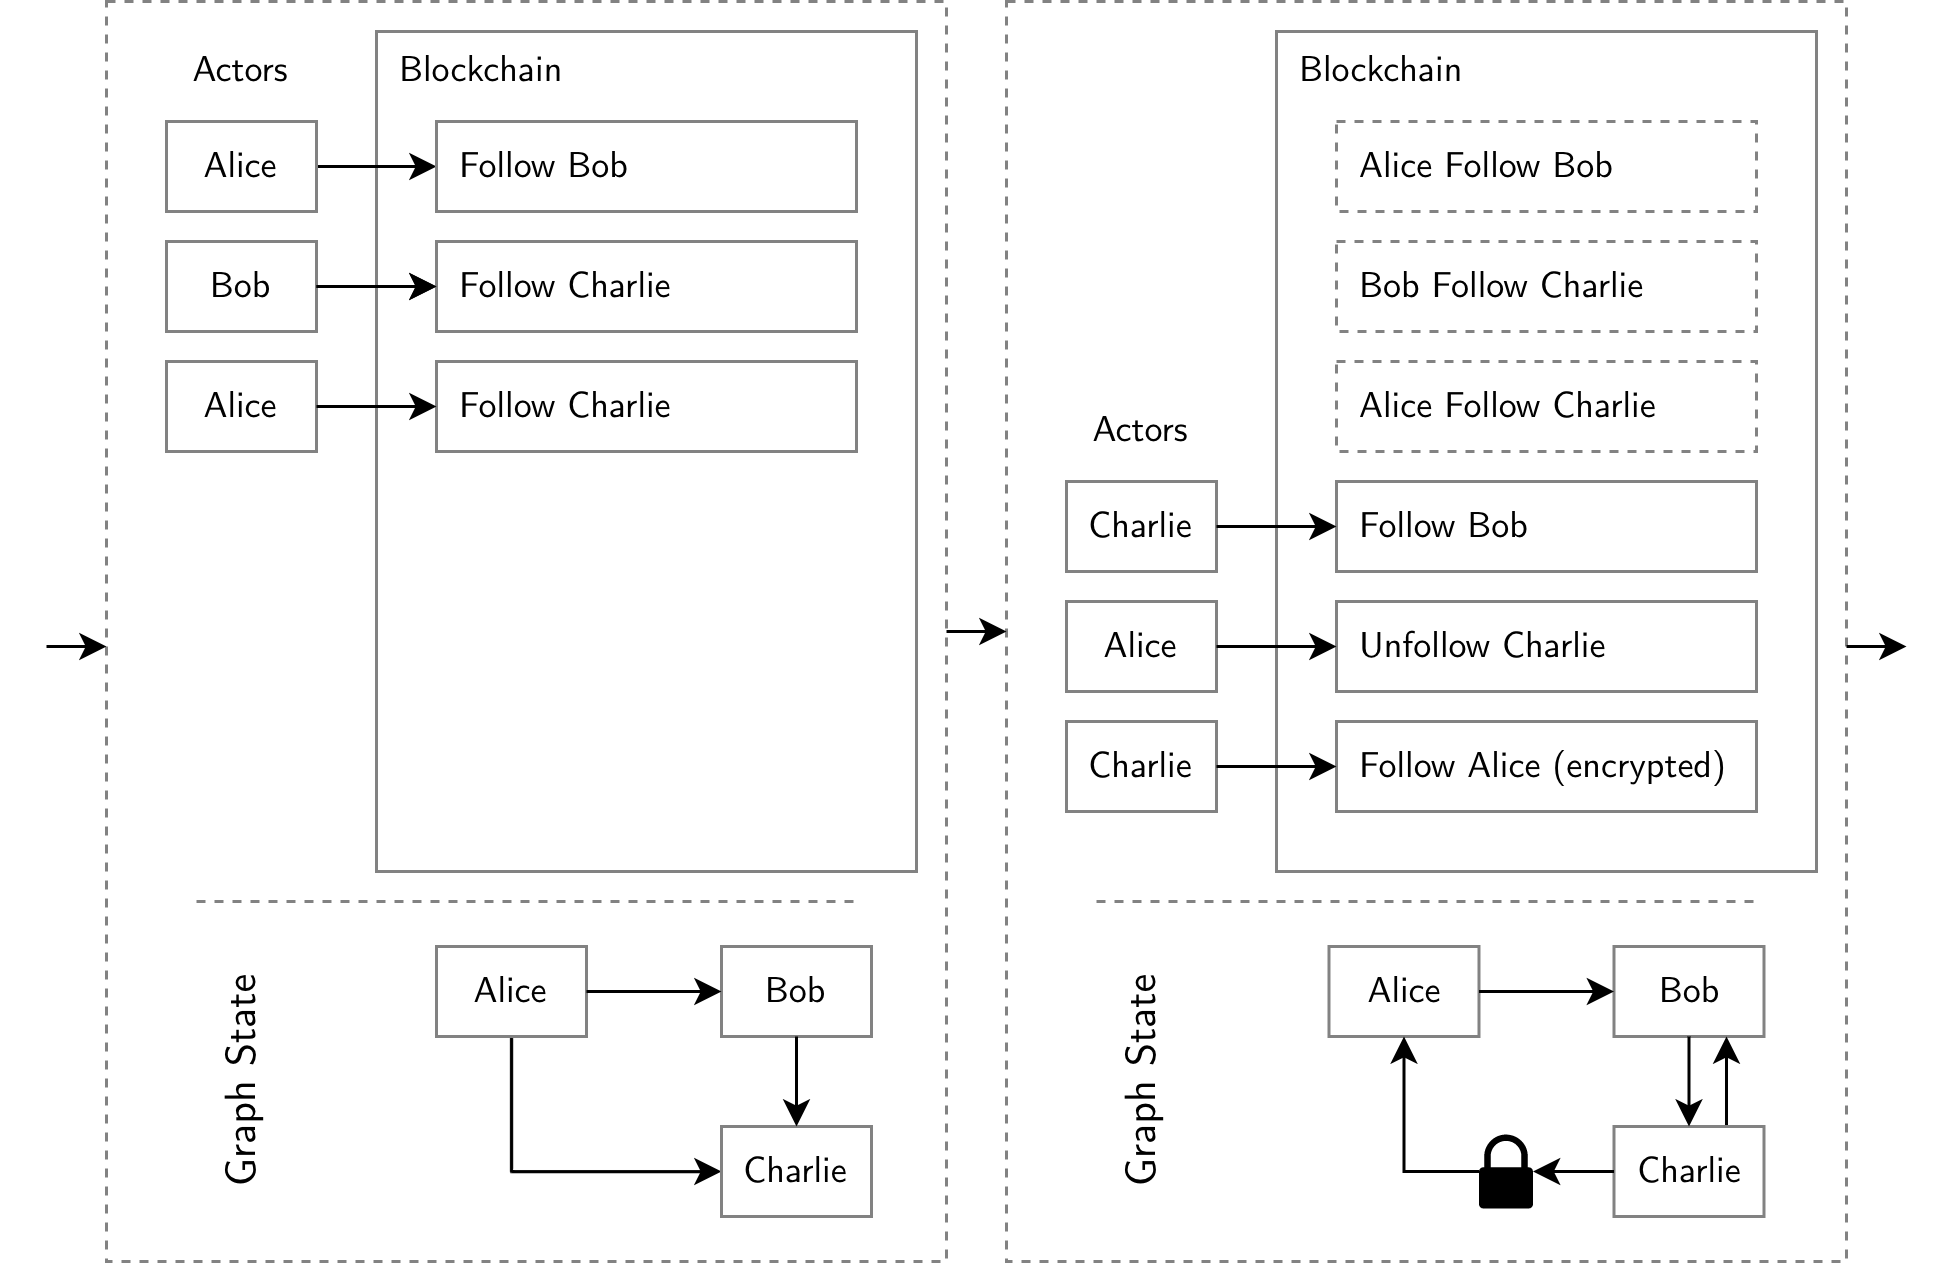
\includegraphics[width=\linewidth]{figures/Graph Change Events.png}
	\caption{Graph Change Events}
	\label{fig:3}
\end{figure}

A series of Graph Change Events are depicted in Figure \ref{fig:3}, along with the
resulting state on the consensus system (notice that the unfollowed friends are no longer
present).

\subsubsection{Privacy}

Graph Change Events always have unencrypted Type and Actor values. Graph Change Events of
type public also have unencrypted \say{Object} and \say{Action} values. Graph Change Events
of type private encrypt the values for \say{Object} and Action. This means that, despite the
Graph Change Event being published to the consensus system, a key is required to interpret
the encrypted values. A user generates a symmetric encryption key for encrypting the private
Graph Change Events data.\footnote{The specification now utilizes asymmetric key pairs to
  generate one-off symmetric keys via a key agreement algorithm. This provides improved
  security and allows for additional use cases while minimizing key management overhead.}
The user can store this encryption key in their wallet or on chain
(see the \say{Key Storage} section).  While private Graph Change Events do not allow outside
observers to read who is being followed, it is still possible to see that the Social
Identity expressed in the Actor field is actively publishing a particular type of event,
which may still convey some level of valuable metadata information to a third party.

\subsubsection{Validation}

Graph Change Events are only partially validated when published to the consensus
system. Type and Actor are validated as part of the publishing process. However, since
Object and Action may be encrypted and unreadable by the consensus system logic, they are
validated by the consumer of the Graph Change Event message. Private Graph Change Events can
be validated only by those who can decrypt the data.\footnote{There may be ways for Social
  Identity addresses to be deterministic. This would provide ways for a user to follow users
  who have not yet joined, but might later join, the network.}$^{,}$\footnote{It might be
  possible to create Graph Change Events where the Object is not a Social Identity.
  Shifting validation to the event consumer would make context available for validation that
  would be unavailable within the constraints of consensus system transaction processing.}

\subsubsection{Sharing}

While public Graph Change Events are fully understandable by everyone, without additional
action, only the Actor user has the ability to interpret their private Graph Change
Events. Users may wish to share their graph with other users, user agents, or third-party
online tools. Sharing is a conceptually simple process, but like many self-sovereign
schemes, ceasing sharing is substantially more complicated.

To share their list of private Graph Change Events with another party, the user can simply
communicate their symmetric key through a secure direct channel. Doing so allows the other
party to read the data, but does not allow them to modify it. The key is used for data
encryption, but does not allow signing new Graph Change Events from that Actor.\footnote{The
  third party would also have to be a delegate with the appropriate permissions on the
  user’s Social Identity, in addition to having the symmetric key, in order to post a valid
  Graph Change Event.} This simple approach, however, is complicated by the need to be able
to cease sharing with a third party.

\subsubsection{Cease Sharing}

To stop sharing private Graph Change Events with a third party, the symmetric key used to
encrypt data on the Graph Change Event is rotated to a new value. No existing Graph Change
Events are changed, but new Graph Change Events will use the new key to encrypt their
private data. While the third party can continue to read the data from before the key
rotation,\footnote{It is impossible to prove that something has been forgotten, thus access
  to old data can be enforced only by the delegate, not the user.} they cannot observe new
changes to the graph, including unfollow Actions of Graph Change Event events for Objects
they previously saw. The ability to revoke access to new Graph Change Events, much like the
ability to revoke access to actions on their Social Identity, ensures that users maintain
control of their graph data and its accessibility across various networks and tools.

\subsubsection{Key Storage}

\begin{figure}
	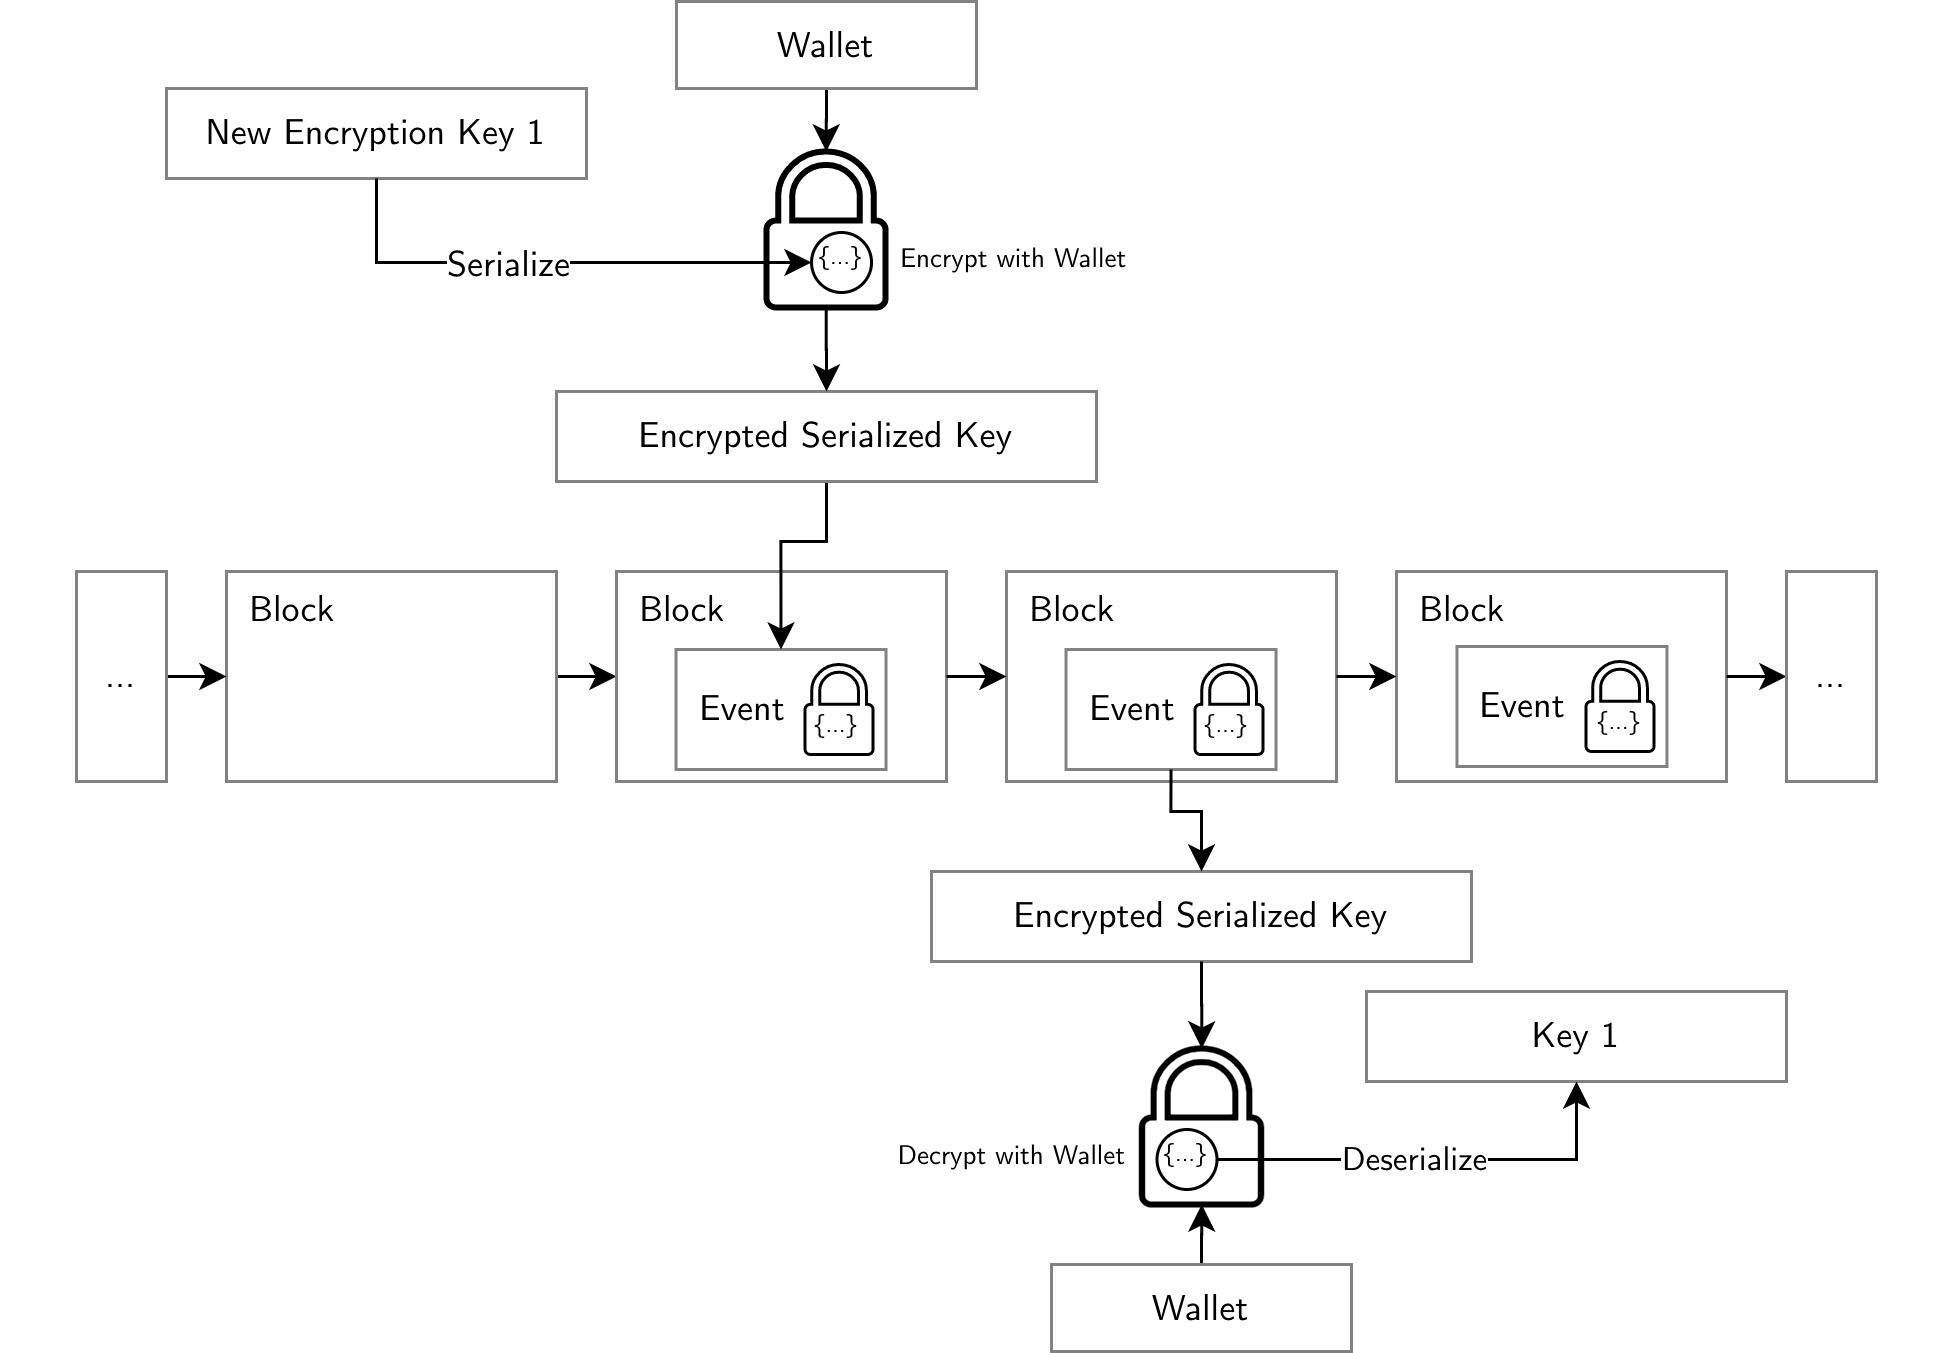
\includegraphics[width=\linewidth]{figures/Key Storage and Retrieval.png}
	\caption{Key Storage and Retrieval}
	\label{fig:4}
\end{figure}

To maintain portability, the keys used to encrypt private Graph Change Events need to be
stored such that they are accessible from multiple devices. These keys can be serialized and
encrypted and stored on the consensus system. The wallet has a few options for encrypting
data, such as using the private key to deterministically generate a key useful for
encryption\footnote{Used in MetaMask.\cite{metamask_doc}} and EIP-2844.\cite{eip2844} Each
key is then able to be retrieved and decrypted by the wallet as needed.

\section{Messaging}\label{sec:messaging}

DSNP addresses messaging as a first-order concept so users can communicate with each other
through a social graph. Posts, replies, reactions/likes, and direct messages are all
examples of different message types today in social networks. To enable messaging, several
key components are needed:

\begin{samepage}
	\begin{description}
		\tightlist
		\item[Announcement:]
		      A structure representing that a message exists
		\item[Announcement Metadata:]
		      Key metadata embedded in an announcement allowing
		      message verification and simple correlation of related messages
		\item[Content:]
		      Detailed data containing the message text, additional metadata, and media links
	\end{description}
\end{samepage}

Combined, these components allow for a minimal model of most current social network
messaging use cases, including broadcast and directed messaging types, as well as public and
private messaging types. They may also be adapted to Layer 2 strategies to manage scale and
cost. An example of this is Batch Message Announcements, as described in Appendix
\ref{app:batch_message_announcements}.

\subsection{Announcements}\label{sec:announcements}

Announcements allow users to become aware of messages in different ways, depending on the
type of message. Email uses SMTP to communicate between persistent nodes. Existing
balkanized social networks perform this task by directly updating their internal systems.
In a decentralized network without unique persistent nodes, however, the difficulty in
making Announcements is twofold. First, the route to the receiver is not fixed; a user may
be in multiple locations or using multiple devices. Second, the receiver may have only
intermittent connectivity, so the network needs to maintain Announcements until the receiver
is available. In addition, in the social media case, users expect that messages sent today
will persist for followers added in the future, indefinitely.

These constraints lead to a system of Announcements that are anchored to the consensus
system.  This system allows message recipients to replay messages as necessary or to monitor
the system for incremental Announcements as they are created. To accomplish this task,
Announcements include a minimal set of essential metadata that can be used to quickly filter
messages needed for a given user.

\subsection{Announcement Metadata}\label{sec:announcement_metadata}

The protocol models a flexible Announcement data structure. All Announcements have at least
four key attributes, but the format allows extensions to this data set to accomplish
additional use cases. The four key attributes are:

\begin{samepage}
	\begin{itemize}
		\tightlist
		\item
		      Message Type
		\item
		      Social Identity that is the source of the message
		\item
		      URI of the content
		\item
		      Hash of the content located by the content URI
	\end{itemize}
\end{samepage}

\begin{figure}
	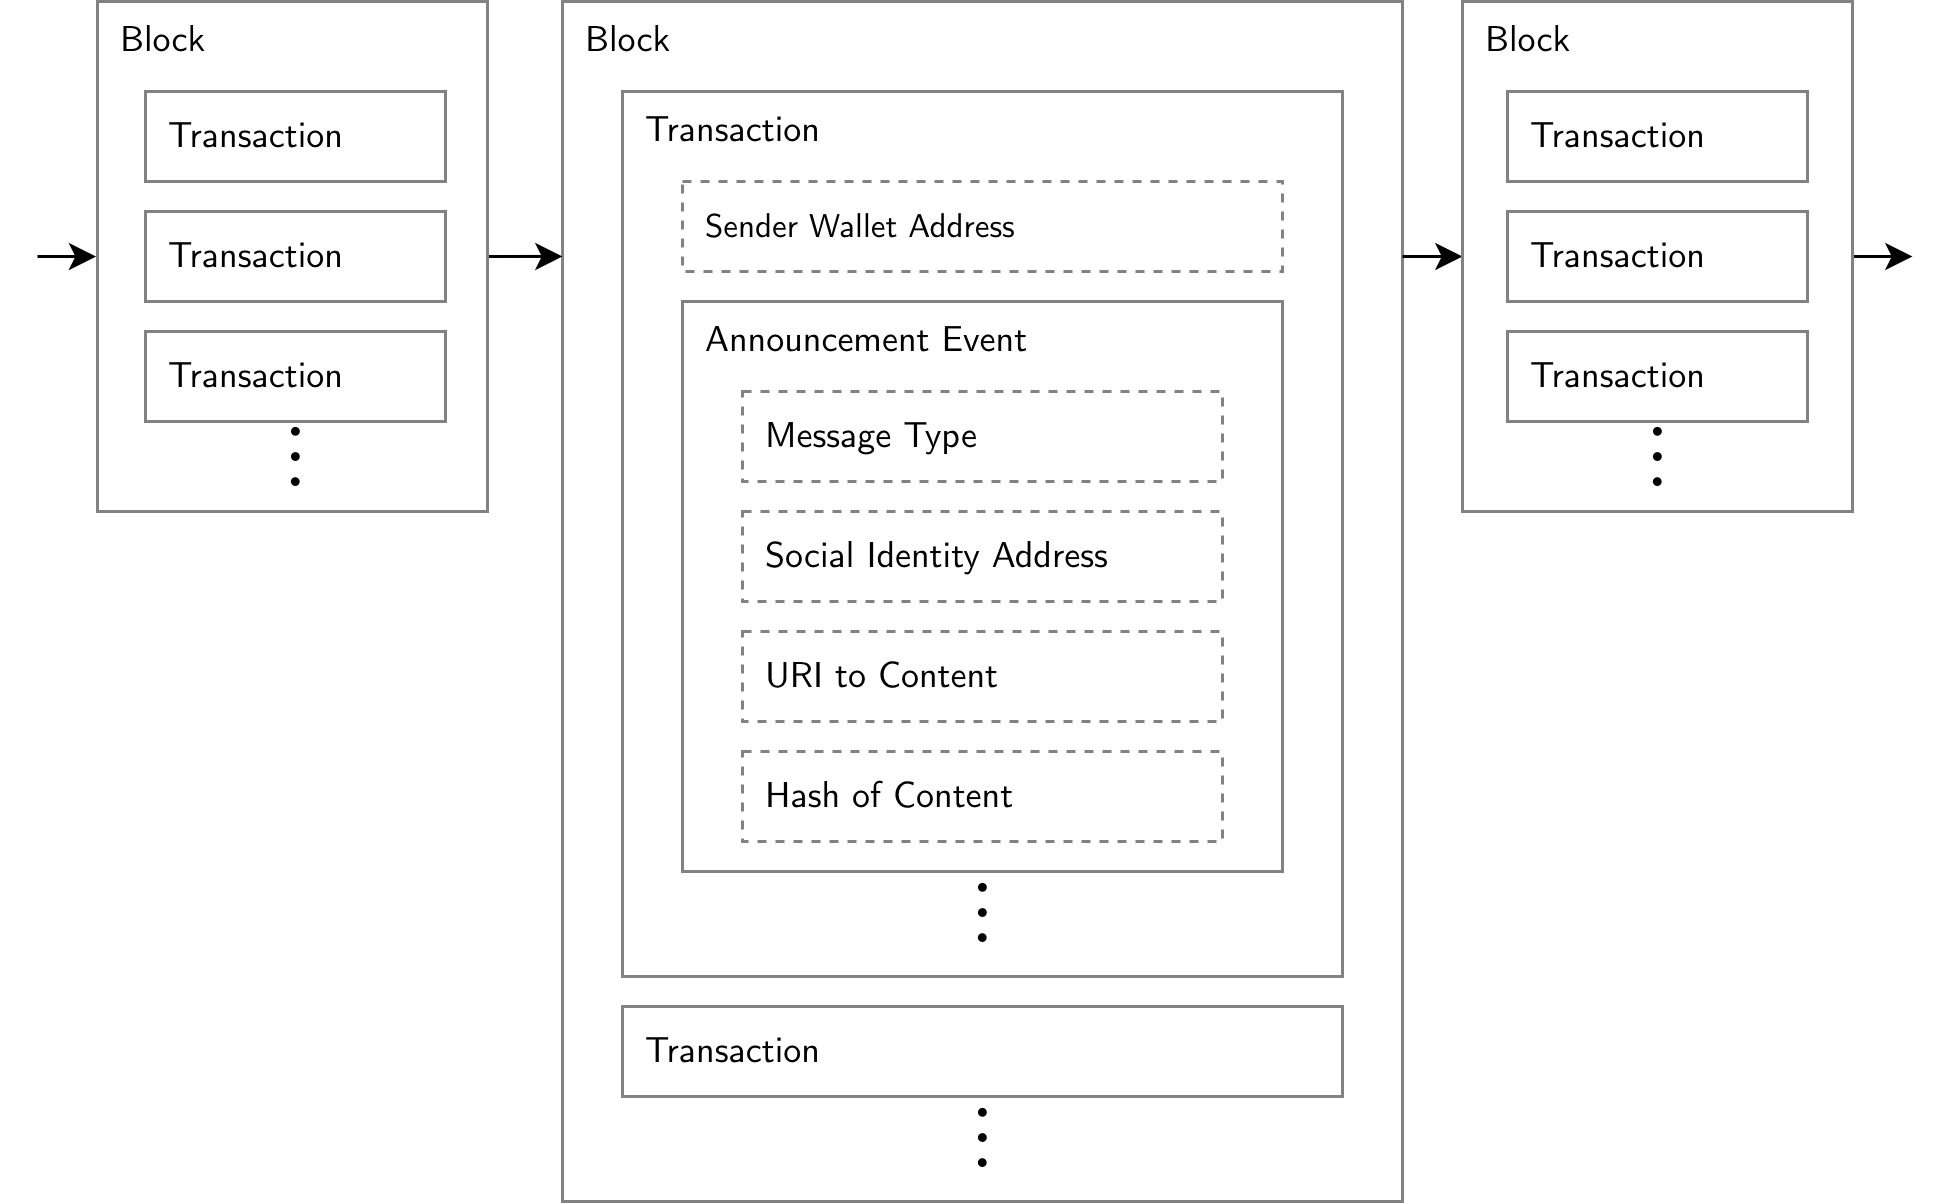
\includegraphics[width=\linewidth]{figures/Announcement Metadata Structure.png}
	\caption{Announcement Metadata Structure}
	\label{fig:5}
\end{figure}

\begin{samepage}
	These key attributes allow Announcements to answer four key questions:

	\begin{enumerate}
		\tightlist
		\item
		      What type of message is this?
		\item
		      Who sent this message?
		\item
		      Where is the content located?
		\item
		      Is the content I am seeing exactly what was originally sent?
	\end{enumerate}
\end{samepage}

The four key attributes defined as metadata on each Announcement answer this set of
questions for all Announcement types, and help prove the validity and authenticity of the
related data.

\subsubsection{What type of message is this?}

Messages are modeled as events on the consensus system. Each Message Type is represented by
a different event. The simplest is a Broadcast message, which has only the four key
attributes already identified for an Announcement. Message Types may define additional
attributes needed for their specific use case.

\subsubsection{Who sent this message?}

As described in the section on Social Identity, the user has the ability to authorize third
parties to take actions on their behalf via the protocol. This means that a valid message
must come from the user's Social Identity, but that the operation may be invoked by the user
or an authorized third party. This allows more flexible use cases, such as delayed sending
and cost shifting. When verifying a message sent in this manner, the consensus system
security mechanism combined with the implementation logic can be used to ensure that only an
authorized party sent the author's message. While authenticating authorship is expected to
be primarily the domain of aggregators or other intermediaries, it is important that any
message recipient be able to directly and independently authenticate message authorship in
order to ensure portability and system integrity.

\subsubsection{Where is the content located?}

Content hosting is assumed, by default, to be the responsibility of the sender. It is,
however, possible for the sender to delegate this responsibility to a third party. The only
criteria for content hosting is that the data should be persistently available and have
unrestricted access for retrieval. The Announcement contains a URI of the content location,
enabling recipients to retrieve the content. The URI is expected to most often be an
HTTPS\footnote{Why not HTTP? Serving HTTP content to HTTPS websites will fail in most
  browsers, but serving HTTPS content to an HTTP website will still work.} URL, allowing
direct access to the referenced content, but any other protocol that is generally accessible
may be substituted. Examples include Swarm or IPFS, with the caveat that protocols not
supported by a recipient's user agent may limit interoperability.

\subsubsection{Is the content I am seeing exactly what was originally sent?}

The Announcement contains a Hash of the content referenced by the content URI. When the
content is retrieved, the retrieved content can be hashed using the same algorithm and
compared with the Hash in the Announcement. Matching Hashes indicate that the content is
valid. To ensure unique hashes between Social Identities, the contents of the message must
include an author property that matches the announcing identity. Content retrieved from a
proxy or cache can also be validated, even when from a different URI, as long as the content
is not transformed by such mechanisms.

\subsection{Content}\label{sec:content}

After a user has received a message Announcement and retrieved and authenticated the
contents of a message, the content must still be interpreted. DSNP is adapting the W3C
Recommendation on Activity Streams\cite{activitypub} to represent content data and
metadata. Only minimal changes to the standard are needed to achieve integration with the
consensus system-related use cases, and the expected changes may be compatible with existing
tools. In addition, this may make it possible to bridge the unified graph emanating from the
protocol and other Activity Stream implementations, as a result of common data models for
content.

Required changes to Activity Streams include enhancements to implement additional data for
certain elements. An example is the Link model in Activity Streams for linking to images.
While content can be authenticated through a chain of hashes or signatures back from
Announcement to the trust of the consensus system, complete validation would require that
the chain of hashes or signatures continue to the images or other data linked in the
content.  \say{Link} is augmented with a hash that can be used to easily verify that the
linked content has not changed.

\subsection{Broadcast and Directed Messaging}\label{sec:broadcast_and_directed_messaging}

As previously described, the Message Type specifies the behavior and ancillary attributes of
a message. Four key Message Types are defined here, though additional types may be created:

\begin{samepage}
	\begin{description}
		\tightlist
		\item[Broadcast:]
		      A message with no recipient
		\item[Reply:]
		      A message with a referent or source message
		\item[Direct:]
		      A message with a public recipient
		\item[Dead Drop:]
		      A message with a private recipient
	\end{description}
\end{samepage}

\subsubsection{Broadcast}

A Broadcast message is an Announcement with no recipient. Users primarily discover these
messages by following the author and monitoring for messages with the author as the
sender. Such messages may also be aggregated into public feeds and presented by
recommendation algorithms. This form of message is analogous to public social media posts.

\subsubsection{Reply}

A Reply message is just like a Broadcast Announcement, but with a referent (\say{In Reply
  To}) message ID. A Reply message Announcement depends on the fact that content Hashes are
unique for any content and Social Identity combination. As mentioned before, the content
needs to include a matching author to validate. Each message may then generate its Hash
before the Announcement is made and can therefore be referred to in an unambiguous
fashion. A Reply Announcement uses this value as the referent message ID. A Reply message
can reference a Broadcast Announcement or another Reply Announcement. This form of message
is analogous to a comment on a public post on a Facebook page. Replies do not need to have
complex content and can be used to represent reactions such as likes or upvotes.

The need for this additional piece of information at the Announcement level instead of in
content metadata is driven by discoverability. Users are often interested in replies to
messages they have already discovered or are otherwise made aware of from Social Identities
they do not follow. By placing the reference message in the Announcement, users can discover
entire subtrees of content related to messages they have already received.  Without such a
mechanism, they would need to monitor all messages on the chain, retrieve the content URL,
and examine it for relevance. At any scale, such actions are prohibitively inefficient.

\begin{figure}
	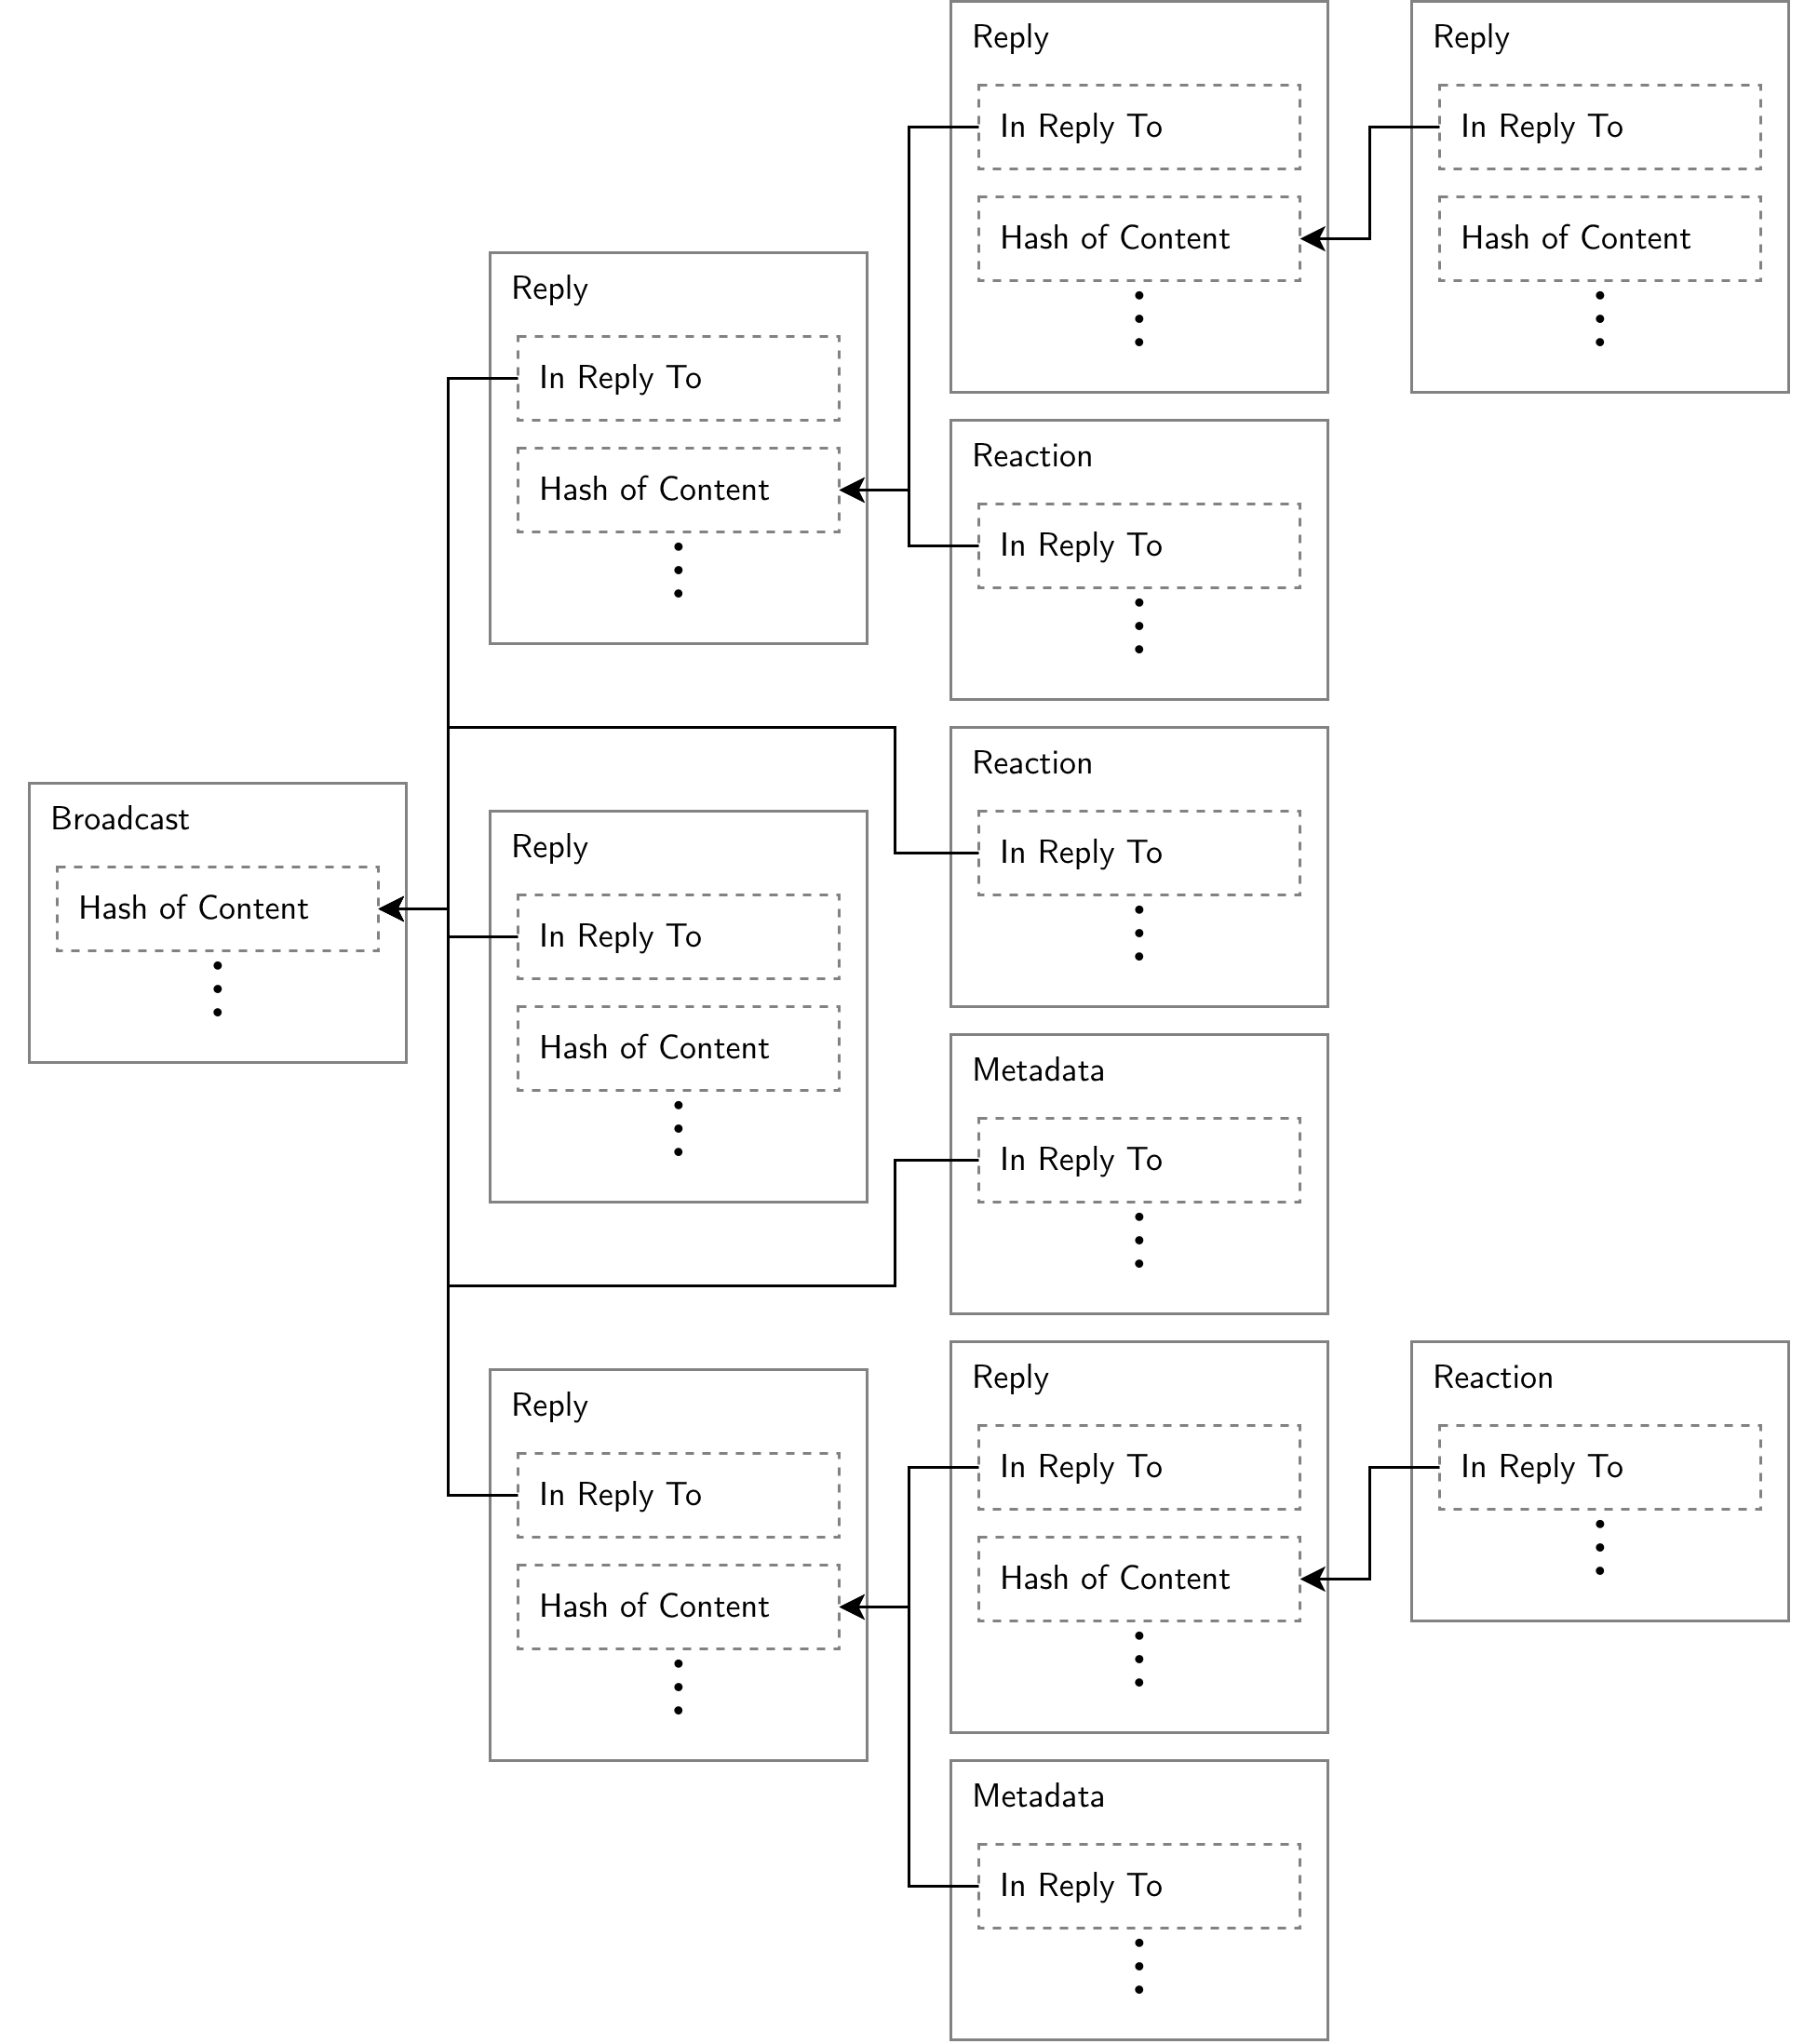
\includegraphics[width=\linewidth]{figures/Message Types and Replies.png}
	\caption{Message Types and Replies}
	\label{fig:6}
\end{figure}

\subsubsection{Direct}

A Direct message is sent to a specific Social Identity. Both the sender and the receiver are
public, although the contents of the message would usually be encrypted. This message is
analogous to an invitation to connect on LinkedIn. One of the ways users discover relevant
message Announcements is by looking for Direct messages sent to their Social
Identity. Friend requests or other cases where a recipient might not otherwise know to look
for message Announcements from the message sender can use Direct messages to establish
communications.

\subsubsection{Dead Drop}

A Dead Drop message is an Announcement that uses a special mechanism, called a Dead Drop
Identifier (DDID), to indicate the recipient of the message, instead of a Social Identity.
The intention is to provide end-to-end encryption and metadata privacy by concealing the
intended recipient, in order to avoid revealing the receiver's private social graph
relationships through metadata analysis. This is analogous to a Twitter direct message,
where outside parties can neither read the message nor even determine that the two parties
are communicating with each other. DSNP extends this protection, preventing service
providers from reading message contents or knowing who is communicating.

Dead Drop Announcements must be addressed with care. The intended recipient needs to know
that the Announcement is for them, but the network must not. One option for a user to
discover a message intended for them with an encrypted recipient field is to attempt to
decrypt every encrypted message on the network. The Whisper protocol from the Ethereum
Foundation uses this model.\footnote{\say{Topics} provide a small amount of difficulty
	reduction, but only at a privacy loss.\cite{whisper-how}} As referenced for Reply
Announcements, this option is prohibitively inefficient at scale.

The protocol uses a novel Dead Drop ID system similar to the dead drops that are a staple
of classic spycraft. For example, Alice places a message under a bench in the park. Anyone
who stumbles upon the message would be unable to identify the intended recipient. Bob,
however, knows the dead-drop location and can privately discover, retrieve, and read the
message.

Classic dead drops have a major logistical issue: The dead-drop location must be known to
both the sending and receiving parties, but not to anyone else. This means the two parties
must have an initial means of communicating before they establish the dead drop. No matter
how secure the dead-drop mechanism is on its own, it relies on the security of the initial
means of communication. Unlike the physical realm, public key cryptography provides a
means to independently derive a common shared secret without prior private
communication.\cite{diffie-hellman1976} Dead Drop Announcements leverage this shared
secret to algorithmically create unique Dead Drop Identifiers that cannot be traced to the
intended recipient.

The identifiers are unique based on each sender-receiver, so each user has a different Dead
Drop Identifier for sending a message to the other. This is analogous to Alice passing
messages to Bob by leaving them under a park bench, and Bob passing messages to Alice by
leaving them in a planter outside the hardware store: Two private, simplex channels with
recipient privacy create a single, duplex channel with recipient privacy. At the event
level, an observer can see that Alice and Bob are both sending messages, but cannot
determine that they are sending messages to each other. If Alice and Bob each run their own
consensus system node for retrieving content, or use nodes not run by a bad actor, they
should also not be susceptible to information retrieval attacks, though timing attacks
exploiting correlation between their activities are not prevented.

\begin{figure}
	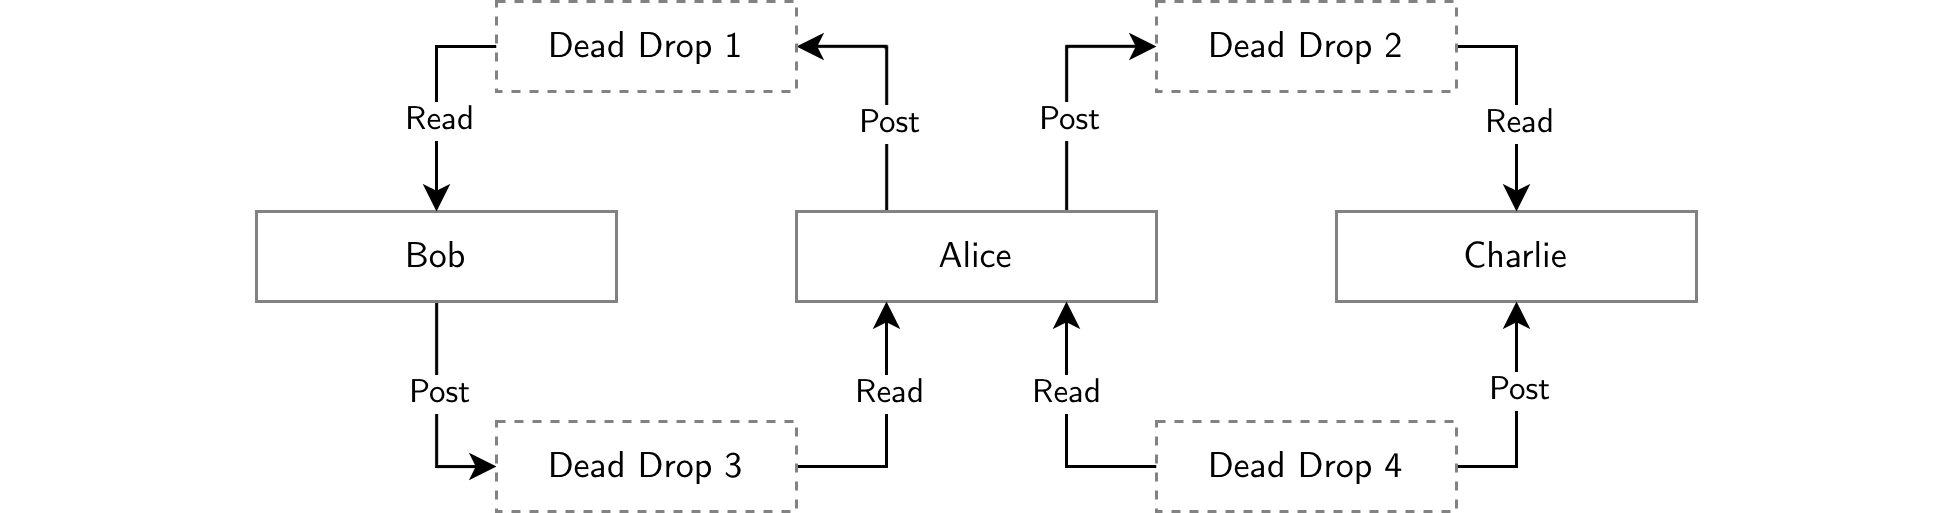
\includegraphics[width=\linewidth]{figures/DDID Flow For Alice with Two Associates.png}
	\caption{DDID Flow For Alice with Two Associates}
	\label{fig:7}
\end{figure}

While Dead Drop Identifiers can be derived without a separate secure communication channel,
there must be some trigger for two users to start listening to each others' DDIDs. This
intent may be communicated out of band, but may also be triggered implicitly or explicitly
by on-chain actions. For example, user agents can choose to monitor DDIDs for all public
followers of a Social Identity, whether perpetually or for a specific period of time after a
follow notification. Alternatively, a Direct message Announcement could be sent from one
user to the other with encrypted content expressing the desire to communicate with DDIDs,
causing both to derive and monitor the relevant DDID values.

\subsubsection{Other Message Types}

The Announcement Message Types are extensible and are a flexible mechanism for adding new
features to the core messaging capabilities of the protocol. For example, spam scoring
services can express a spam score about Broadcast messages by extending Reply messages with
a new Message Type and including scoring data in the Announcement or content. The same
mechanism can be used for other services, such as fact checking, reputation scoring, or
moderation, to add arbitrary metadata to an existing message.

A Message Type may also be constructed to refer to a group of Announcements. This type
enables \say{batching} or Layer 2 Announcements to reach the consensus system in a
cost-efficient structure, while still preserving the authenticity of messages. A simple
Batch Message Announcement structure is described in Appendix
\ref{app:batch_message_announcements}.

Another Message Type common to social media is a Reaction type. Reactions are similar to
Reply Announcements, but with different metadata attached. A Reaction might have a sentiment
value of positive, neutral, or negative, as well as a suggested rendering. The sentiment
allows for simple cross-client display of reactions, while a suggested rendering can be used
to expand the range of emotion for supporting clients.

\section{Batch Message Announcements}\label{app:batch_message_announcements}

A Batch Announcement is an extension of the Broadcast Announcement, and has the same
set of data. It exists to allow the \say{batching} of all Announcement Message
Types. Batch Announcements allow the publication of more than one message
Announcement with a single on-chain Announcement.  These Batch Messages introduce a
new service role called a Batch Announcer, which collects message Announcements and
batches them together. They have some trade-offs versus other Message Types, but
allow substantial scaling increases and cost reductions.

\begin{figure}[h]
	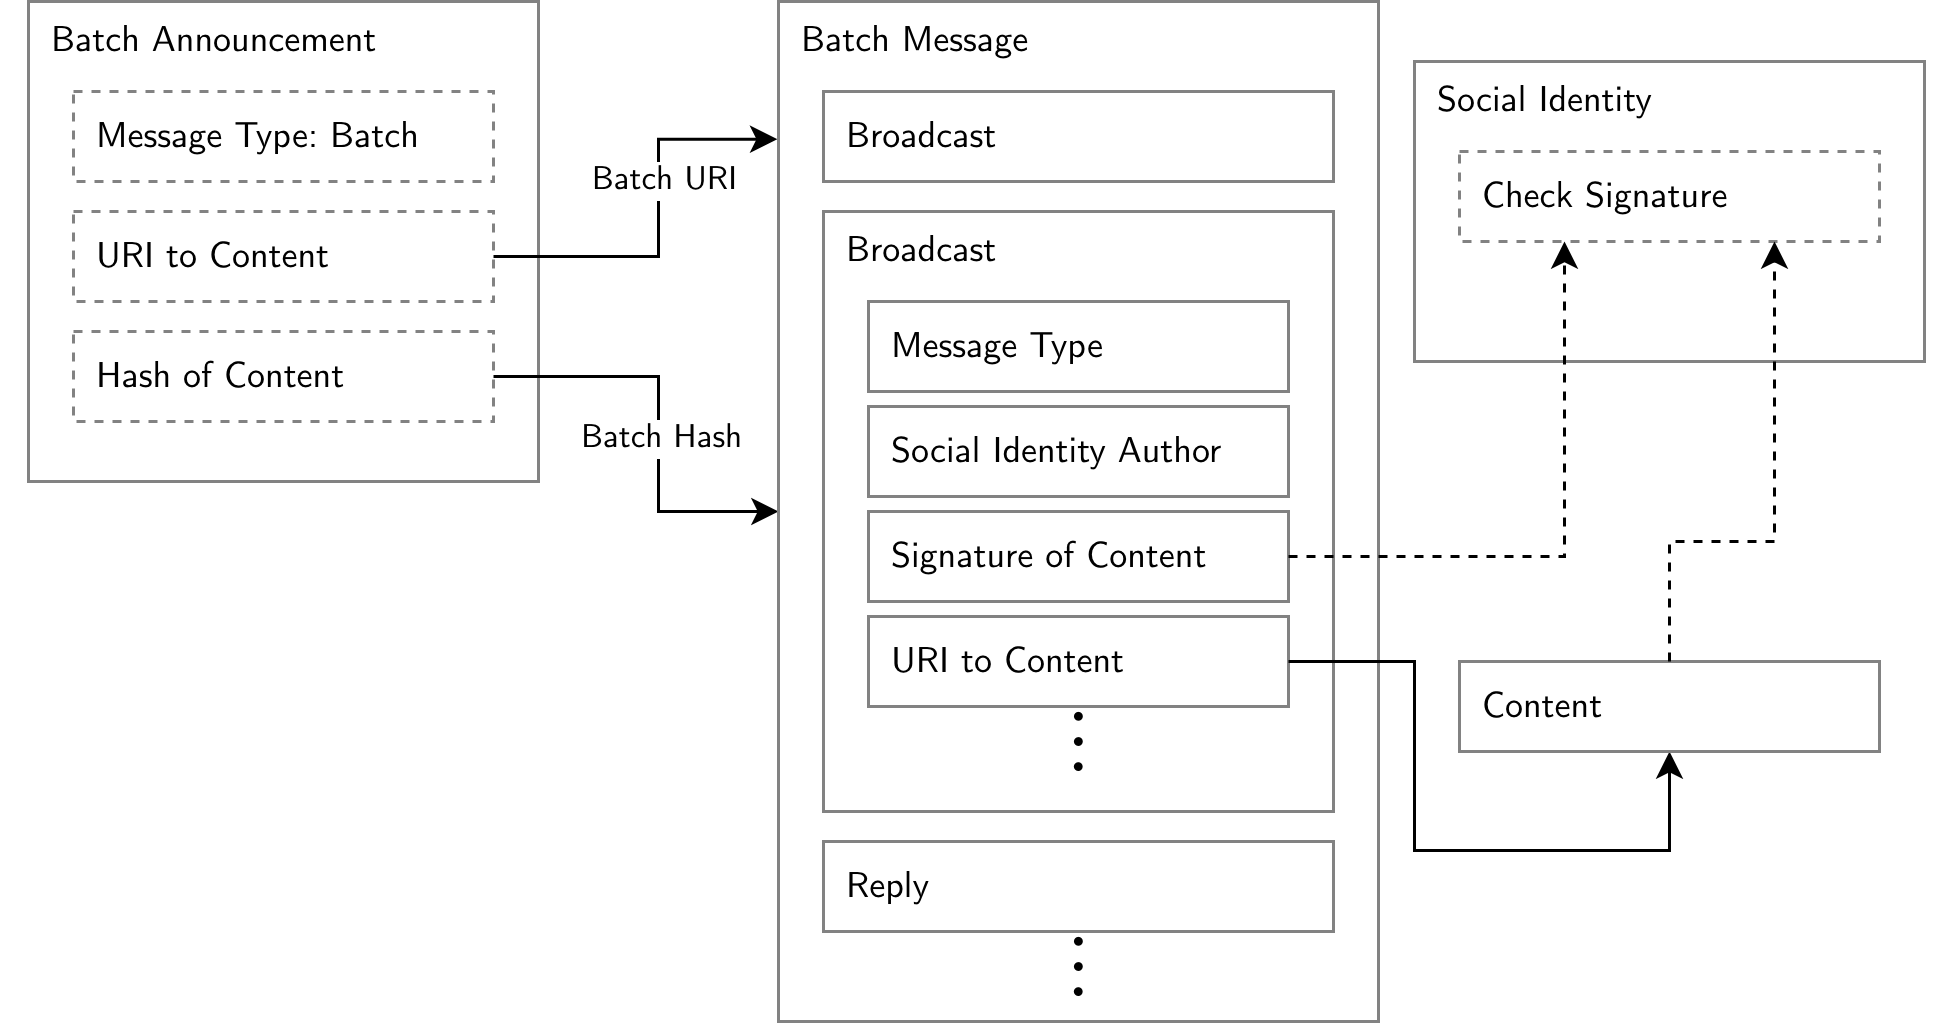
\includegraphics[width=\linewidth]{figures/Batch Message Structure.png}
	\caption{Batch Message Structure}
	\label{fig:9}
\end{figure}

A Batch Announcement has a different Message Type than a Broadcast Announcement, but
otherwise has the same structure. However, the URI for a Batch Announcement always
refers to a Batch Message file, the content of which has a specific file format, and
is an ordered list of other Announcements. Each of the included Announcements has
its complete set of Announcement metadata, including Message Type, Social Identity
source, content URI, content Hash, and any type-specific Metadata (for example, a
Reply Announcement would also have a referent message ID).  Each Announcement also
contains the Social Identity address of the sender and a signature of the URI
content, replacing the signature that would have been used when posting to the
consensus system. The Announcements included in the Batch Message file are not
broadcast directly to the consensus system. However, since each message in the Batch
Message file has a Hash, Social Identity, and signature, and the Batch Announcement
has a Hash of the Batch Message file, authenticity still traces from each individual
user message back to the chain, using techniques such as EIP -1271,\cite{eip1271}
BLS12-377,\cite{el2020} or other similar approaches.

\begin{figure}
	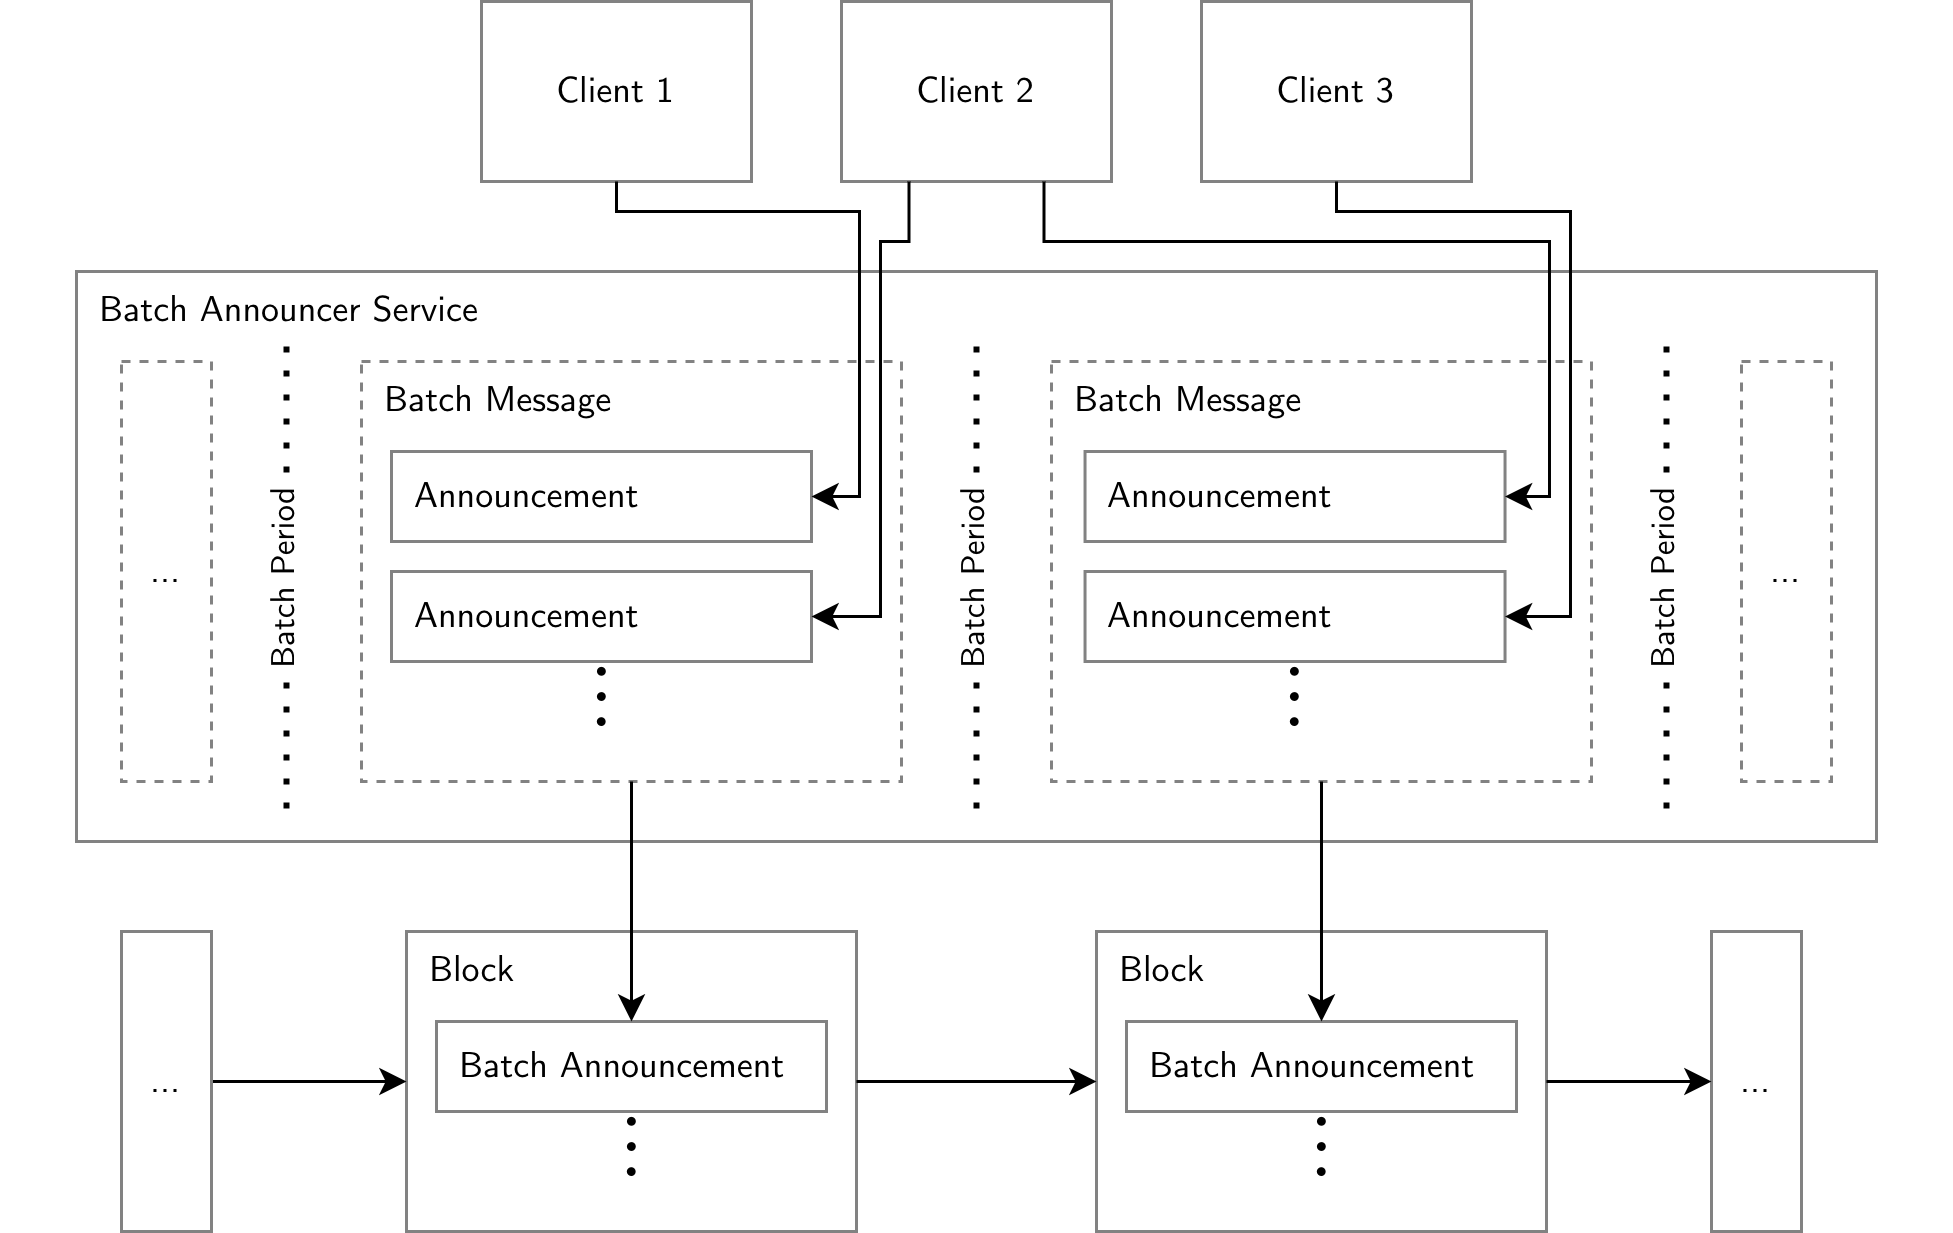
\includegraphics[width=\linewidth]{figures/Example Batch Process.png}
	\caption{Example Batch Process}
	\label{fig:10}
\end{figure}

This approach has a number of trade-offs. Benefits include lower cost and better
scaling while maintaining authenticity. Drawbacks include increased complexity and
the off-chain nature of messages referenced by Batch Messages. Increased complexity
comes from the additional indirection used by Batch Messages. However, as volume
increases, most clients will use dedicated content indexing services, which should
have no issue with indexing Batch Messages. Potential latency comes from Batch
Announcers only periodically posting Batch Announcements. The off-ledger nature of
referenced messages can be mitigated by Indexers and other consensus system watchers
replicating or caching Batch Message files.  While a file can be removed, the
existence of the Batch Message is listed on the chain, providing evidence that a
file previously existed and allowing any file copy to be verified for authenticity
against the listed Hash.

Batch Messages are another example of the flexibility and extensibility of the
protocol, enabling implementation on cost-sensitive consensus systems including
sidechain or other Layer 2 blockchain solutions.  Users have the option to publish
Announcements directly or through an Announcement service. Batch Announcements work
in cooperation with, not as a replacement for, other Message Types, while providing
orders-of-magnitude scaling increases and cost reductions.

\section{Conclusion}\label{sec:conclusion}

This paper has proposed a protocol for creating a unified, universally accessible,
decentralized social graph and an associated ecosystem of software services and
applications. A modern social media company is highly complex, with many different
components requiring a wide variety of deep expertise. From technical components such as
software clients, caching services, and recommendation engines,\cite{hashemi2017} to more
business-oriented concerns such as moderation, advertising sales, and regulatory compliance,
each piece is a critical component of the network. This protocol enables coordination
between services to build the complex ecosystem required to sustain modern social media
without the liabilities of centralization. The next step is to create a comprehensive
protocol specification leveraging the significant technical work already completed.

Creating a complete system with so many components can be difficult when all functionality
must occur inside a single organization. By unbundling the social network, an entire
ecosystem can be created to operate at global scale and allow a diverse
array of experts to address the pressing challenges created by malicious actors in the
network. With a public broadcast model of protocol events, new services can be created to
provide simple interfaces and data layers to create and consume data. These SaaS (Software
as a Service) tools can provide an infrastructure layer that clients can leverage in unique
combinations for different use cases. Figure 8 illustrates a hypothetical ecosystem of
independent components that leverage the protocol to create a complete social networking
system.

\begin{figure}
	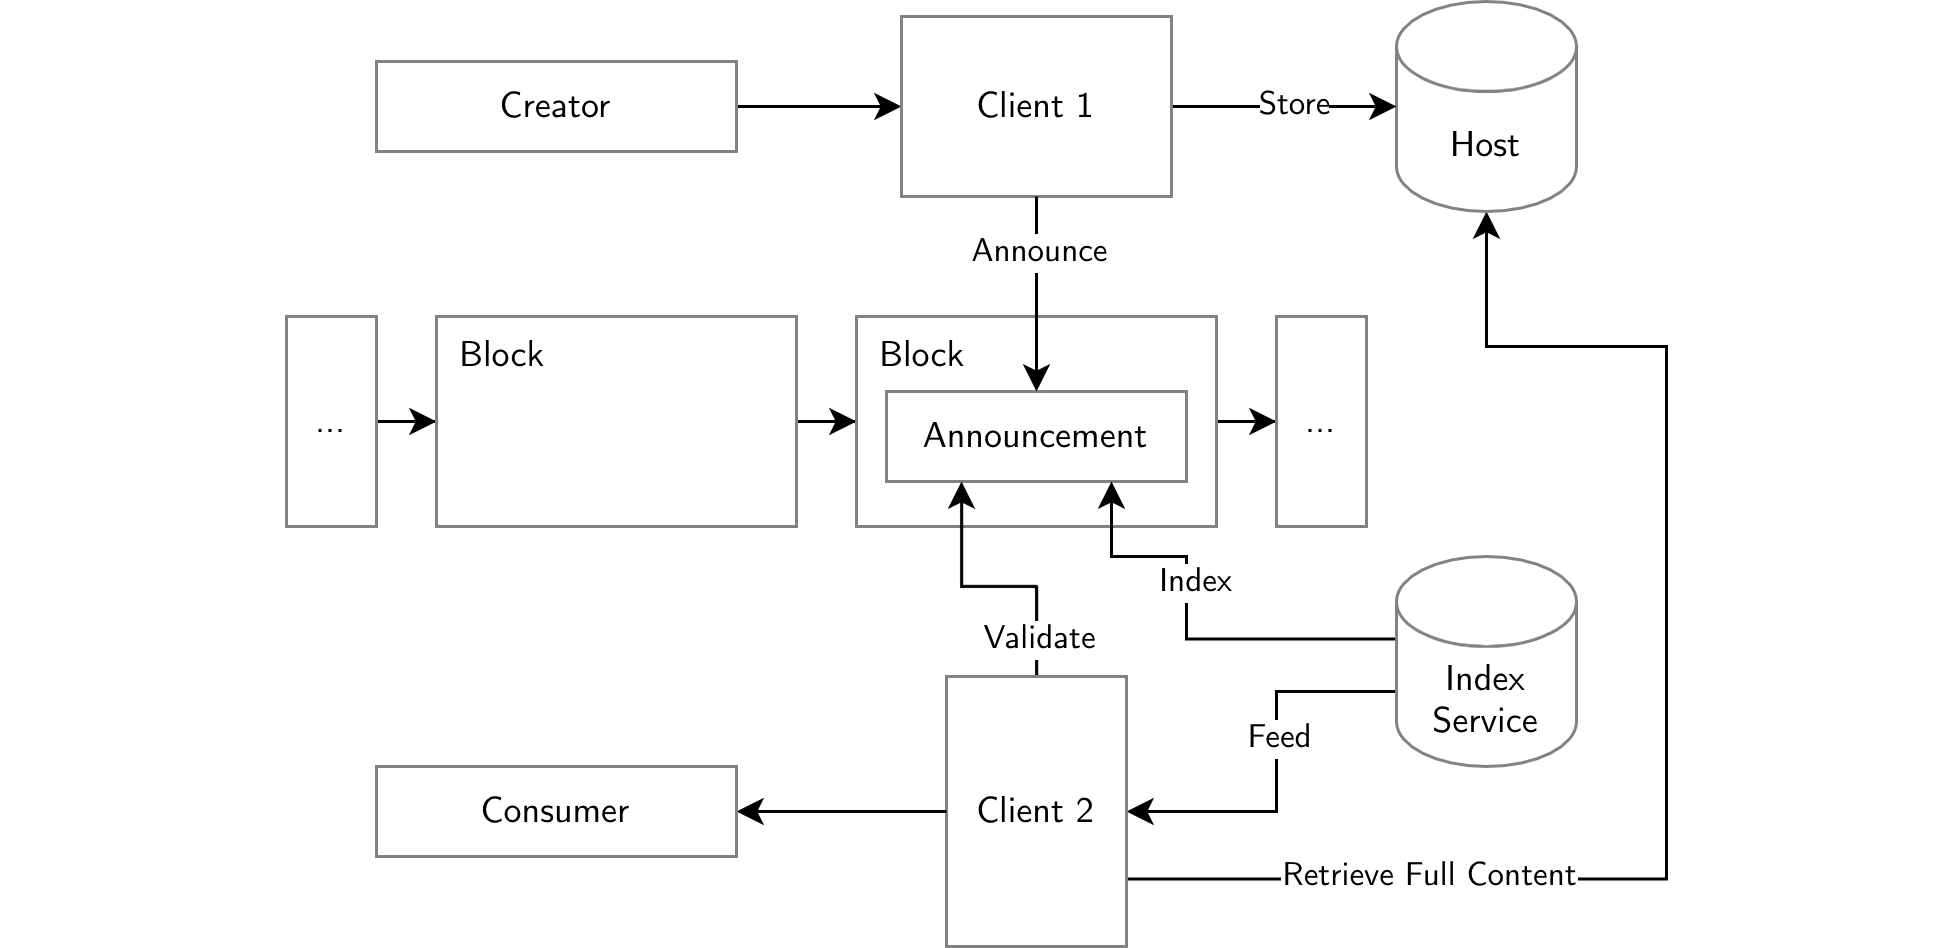
\includegraphics[width=\linewidth]{figures/SaaS Ecosystem.png}
	\caption{SaaS Ecosystem}
	\label{fig:8}
\end{figure}

A diversity of approaches, leveraging the interoperability of common data formats and
discovery, minimize the effort to create new experiences. Graph indexing services can take
on the load of parsing and storing graph events from the consensus system to provide easy
access to graph data, including mechanisms to handle encrypted events. Content indexing
services can enable content feed building, message threading, search results, trending
topics, or caching, and, since all Announcements provide the information needed to
authenticate the content, can combine trust and convenience. Content moderation and fact
checking can be provided by multiple separate services for different use cases or interest
groups, enabling more reliable, comprehensive, and transparent moderation. Given the open
nature of the network, developers can offer different revenue models that can exist side by
side, such as advertising, subscription, or direct payment, while allowing all experiences
to interoperate directly.

The protocol allows for the same underlying information to be available to everyone
independent of intermediaries. Separating responsibilities encourages competition while
better aligning incentives with user interest. The range of possibilities is difficult to
predict, but by ensuring user data control and decentralizing the interaction model, the
protocol allows for an entire ecosystem of participants to innovate and flourish.

\nocite{0xwhitepaper}
\nocite{al-dahhan2019}
\nocite{al-dahhan2019}
\nocite{ateniese2006a}
\nocite{bünz2020}
\nocite{cheng2020}
\nocite{diebold2017}
\nocite{eip1078}
\nocite{eip173}
\nocite{eip712}
\nocite{ethereumyellow}
\nocite{ge2019}
\nocite{gnosissafe}
\nocite{green2018}
\nocite{henry2018}
\nocite{json-web-encryption}
\nocite{nacl}
\nocite{nakamoto}
\nocite{omara2020}
\nocite{openzeppelin}
\nocite{pirk}
\nocite{raikwar2019}
\nocite{swarm}
\nocite{ugander2011}
\nocite{unilogin}
\nocite{whisper}
\nocite{williams2019}

\printbibliography

\end{document}
